\lettrine[lines=3]{P}{}rocedurally generating 3D models of plant-life is a challenging task, largely due to the complex branching structures and variation between different types of plant species. Up until recently, all assets within 3D graphics applications either had to be sculpted using 3D modeling software or scanned using photogrammetry, laser triangulation or some form of contact-based 3D scanning. These methods are still used today but tend to be very time consuming and extremely costly. With the increase in computational power over the last few decades more emphasis has been placed on the use of procedural generation. Which can be used to create complex structures such as terrain, architecture, sound and 3D models with far greater speed than previous techniques, and often much better realism than would be possible with artists. Plant-life stands as a challenge due to the thousands of species, each with their unique structure and features. It is difficult to define a system that can represent them all in a way that is simple, understandable and accurate. The Lindenmayer System (L-system) stands as a solution to this problem, it was originally developed by Aristed Lindenmayer as a method of representing the development of multicellular organisms \cite{lindenmayer1968mathematical}. This has since gained popularity in the area of procedural generation and has been adapted to represent different types of structures. L-systems have been adapted to represent plant-life, such as trees, flowers, algae, and grasses. Whilst still applying to non-organic structures such as music, artificial neural networks, and tiling patterns \cite{Prusinkiewicz1989}.\\

The L-system in its most basic form is a formal grammar that contains a set of symbols or letters that belong to an \textit{alphabet}. The alphabet is used to create a starting string known as the \textit{axiom}, as well as a set of production rules. The production rules are applied to each symbol within the axiom string, each rule dictates whether or not the symbol can be rewritten and what they will be rewritten with. In essence, an L-system uses the set of production rules to generate a resulting string of symbols which follow those production rules. The resulting strings' meaning can then be interpreted in a way that best fits what it is trying to represent. In this case, the string can be interpreted to generate a model of a plant. This thesis develops upon the L-system concepts described by Przemyslaw Prusinkiewicz and Aristid Lindenmayer to procedurally generate structures of plant-life in real-time. The L-system grammar allows the structure of a plant to be described in a human-readable, formal grammar. The grammar can be used to specify variation in shape, size, and branching structure within a particular species. Furthermore, this thesis will also investigate the use of a parameterised L-systems to provide physical properties using string rewriting. Which in turn will enable the animation and physical behavior of the plant that it generates, thus making it possible to simulate external forces such as gravity and wind.\\

This chapter will describe the motivations behind this research and how it can be used to improve the procedural generation of plant-life in 3D applications. It will then introduce the concepts of procedural generation, rewriting systems and formal grammars. Briefly describing how procedural generation can be applied to the development of plant-life through the use of rewriting systems. Furthermore, this chapter will provide sufficient background as to the use of formal grammars as a means of describing complex L-system languages. Finally, there will be an outline as to the structure of this thesis, and how this research will be conducted.


\section{Motivations}

L-systems have been talked about and researched since its inception in 1968 by Aristid Lindenmayer. Over the years it's usefulness in modeling different types of plant life has been very clear, however its presence has been quite absent from any mainstream game engines and graphics applications for the most part, these engines relying either on digital artists skill to develop individual plants or on 3rd party software such as SpeedTree. These types of software use a multitude of different techniques however their methods are heavily rooted in Lindenmayer Systems. 
 
One of the most time consuming parts for digital artists and animators is creating differing variations of the same piece of artwork. In most games and other graphics applications environment assets such as trees, plants, grass, algae and other types of plant life make up the large majority of the assets within a game, and creating a plant asset can take a skilled digital artist more than an hour of work by hand, The artist will often have to create many variations of the same asset in order to obtain enough variation that a user of that graphics application would not notice that the asset has been duplicated, if this is multiplied by the number of assets that a given artist will have to create or modify, there is an incredible number of hours that could have potentially been put to use creating much more intricate assets. In addition to this, it is also important to note that graphics assets are then stored in large data files, describing the geometry and textures and other information. If we require three very similar plants, we have to store three separate sets of data. Procedurally generating plants can avoid this wasteful data storage entirely, instead a relatively small L-system description can be stored which can be used to procedurally generate all the required geometry and other information during the execution of the program.\\

The L-system can not only procedurally generate the geometry of the plant-life but can also generate parameters physical properties of the plant inself such as the weight and flexibility of branches as well as its wind resistance and many other important information that can be used to simulate or animate the motion of the plant under various forces.  

\section{Introduction to Procedural Generation}

Procedural generation is used in many different areas and applications in computer graphics, particularly when generating naturally occurring structures such as plants or terrain. An effective procedural generator is capable of taking input in the form of a relatively simple description of what it should be generating, its job is then to computationally generate the structure in a way that is accurate to the description given. Currently, there are three main methods for procedurally generating models of plant-life, these are genetic algorithms \cite{haubenwallner2017shapegenetics}, space colonisation algorithms\cite{juuso2017procedural} and L-systems. The genetic algorithm and space colonisation algorithms are similar in that they require the overall shape of the plant to be described by simple 3D shapes, the algorithm then creates a branching structure that matches these shapes. The limitation of these methods is that the 3D description is not very specific and although it can get good results for trees, it may not be able to generate different types of plant-life, such as flowers. The L-system, on the other hand, relies on a method of string rewriting, whereby the rewriting is based on a set of production rules to generate a string of symbols that obey those rules. A separate system can later interpret this string to create the model. The L-system procedural generation, therefore, has two separate systems within it, one of string rewriting and one of interpretation of the generated string. This makes it quite easy for the same L-system to generate very different results based upon the interpretation.\\

Plant-life can have very complex and seemingly random structures, however, with closer observation, trees of a similar species have obvious traits and features. For instance, a palm tree has long straight trunks with long compound leaves exclusively near the top, branching in all different directions. Comparatively a pine tree has a long straight trunk with many branches coming off in different directions perpendicular to the ground, from its base to the top of the trunk. These are two very different species of trees, the palm belongs to the Arecaceae family, whereby the pine belongs to the Pinaceae family. They look different, however, they share very similar properties, such as their long straight trunks. The challenge behind the procedural generation of plant-life is providing a human-readable grammar that describes in sufficient detail, how to generate a 3D model. Whilst allowing for randomness and variety within the generation process, such that variations of a particular species can be generated without repetition. The grammar for procedural generation should also be relatively straightforward and intuitive, and must accurately represent what it is going to generate. Furthermore, the description must not be limited to only known species of trees, as some graphics applications may require something other-worldly.

\section{Introduction to Rewriting Systems}

Rewriting systems are the fundamental concept behind L-systems. In their most basic form, rewrite systems are a set of symbols or states, and a set of relations or production rules that dictate how to transform from one state to the other \cite{prusinkiewicz2012algorithmic}. Using these state transitions it's possible to generate complex structures by successively replacing parts of an initial simple object with more complex parts. Rewrite systems can be non-deterministic, meaning that there could be a transition that depends on a condition being met or on neighbouring states. Using this rewriting concept any preceding state can rely upon some conditions necessary for transformation. If the condition is true the state will be rewritten, otherwise, it will remain the same, and will be checked in the next rewriting stage. A graphical representation of an object defined in rewriting rules can be seen below in figure \ref{snowflake curve} below, called the snowflake curve proposed by Von Koch \cite{koch1906methode}.

\begin{figure}[htbp]
	{\centering
		\setlength{\fboxrule}{1pt}
		\vspace{7px}
		\fbox{
			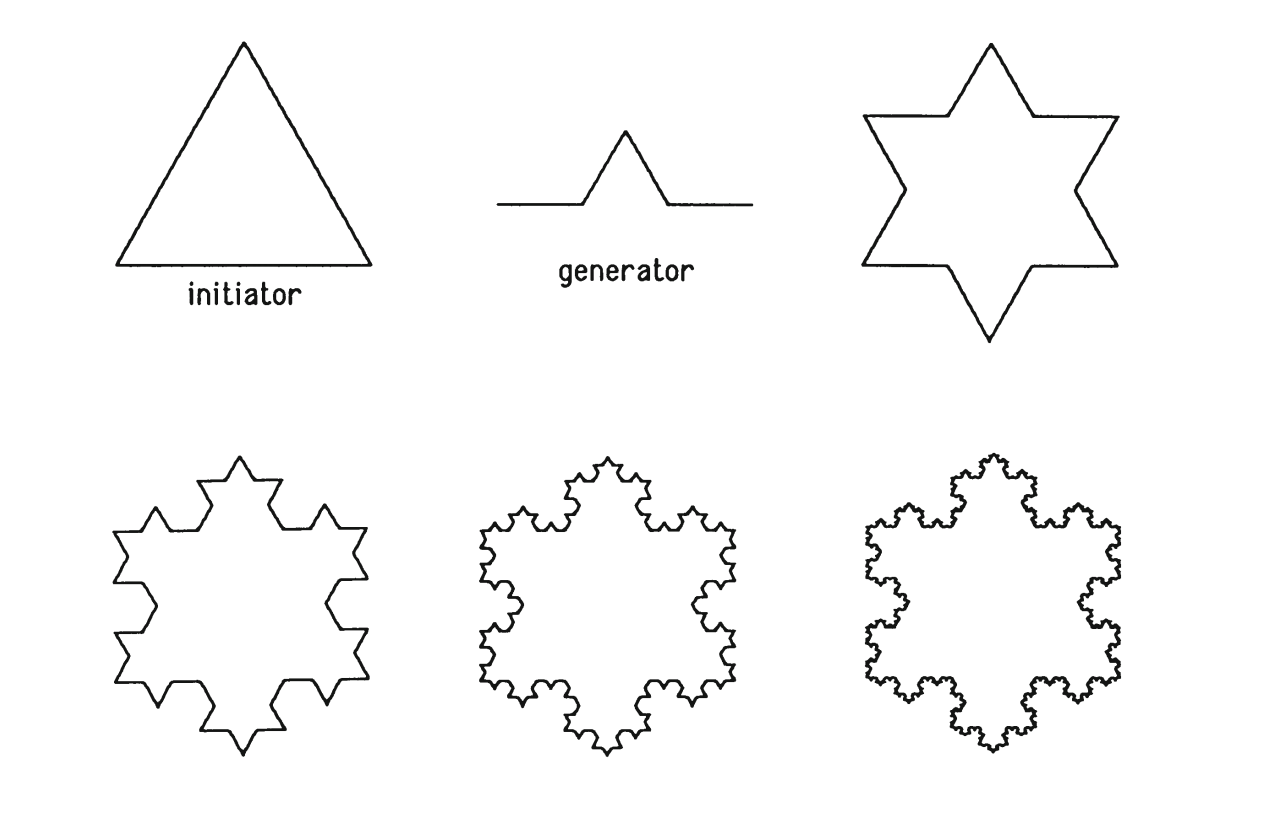
\includegraphics[scale=0.3]{Diagrams/snowflakeCurve.png}
		}
		\caption{Construction of the snowflake curve\cite{prusinkiewicz2013lindenmayer}.} \label{snowflake curve}
	}
\end{figure}
\FloatBarrier

\noindent
The snowflake curve starts with two parts, the initiator and the generator. The initiator is the initial set of edges forming a certain shape, whereas the generator is a set of edges that can be used to replace each edge of the initiator to form a new shape. That new shape then becomes the initiator for the next generation, where each edge is again replaced by the generator. The result is a complex shape similar to that of a snowflake. The initiator, generator concept is a graphical representation of how rewriting systems operate, rather than the initiator and generator being a set of edges they are instead represented by a set of symbols or strings.

\section{Introduction to Formal Grammars}

In the context of computer science, a grammar is defined as a set of rules governing which strings are valid or allowable in a language or text. They consist of syntax, morphology, and semantics. Formal languages have been defined in the form of grammars to suit particular problem domains. It is natural for humans to communicate a problem or solution in the form of language, it is intuitive to use a language to describe the desired outcome when dealing with the procedural generation of plant-life. In the past, formal grammars have been used extensively in computer science in the form of programming languages in which humans can provide a computer with a set of instructions to carry out to gain an expected result. The challenge is to create a  grammar in the form of a rewriting system that facilitates the procedural generation of plant-life. A rewriting system such as the L-system operates in a way that is consistent with a context-free class of Chomsky grammar \cite{chomsky1956three}, similar to that of the programming language ALGOL-60 introduced by Backus and Naur in  1960\cite{backus1960report}. In figure \ref{chomsky grammars} below, two types of L-system grammars overlap the classes of Chomsky grammars, the OL-system, and the 1L-system. The details of these two systems will be discussed in detail chapter \ref{l-system chapter}, but in summary, 0L-systems are grammars that can represent a context-sensitive Chomsky grammar but generally tend to be context-free, the main difference between the 0L-system and the 1L-system is that 1L-systems can be recursively enumerable. Furthermore, a 1L-system can represent any 0L-system, therefore, 1L-system languages tend to be more complex and verbose when compared to 0L-systems, this creates a trade-off between a more powerful and complex language or a less powerful but simpler language. 

\begin{figure}[htbp]
	{\centering
		\setlength{\fboxrule}{1pt}
		\vspace{7px}
		\fbox{
			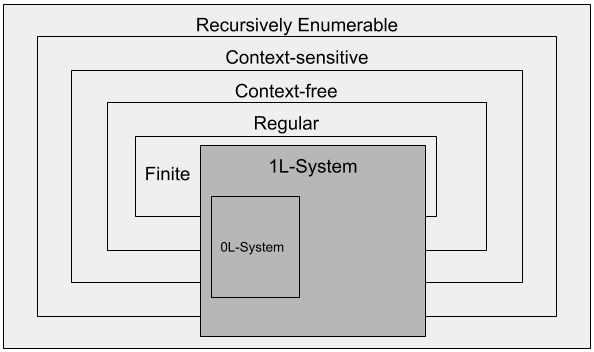
\includegraphics[scale=0.5]{Diagrams/ChomskyGrammar.png}
		}
		\caption{Diagram of the Chomsky hierarchy grammars with relation to the 0L and 1L systems generated by L-systems.} \label{chomsky grammars}
	}
\end{figure}
\FloatBarrier

\section{Structure of Thesis}

This thesis begins by delving into the underlying concepts of L-systems. This starts by defining the simplest type of L-system named the DOL-system, it also goes into detail about how they can be interpreted to produce a graphical representation. This will lead to the formal definition of more complex types of L-systems such as the parametric L-system, which this thesis mainly focuses on. In conjunction with this, the L-system chapter will talk about some of the major features and improvements which can be used to aid the procedural generation of plant life. 

The next major part of the thesis will focus on the L-system rewriter implementation, this includes the definition of the grammar and syntax for a parametric L-system. This includes the process of string rewriting, as well as computationally understanding the L-system grammar using lexical analysis, parsing and the string rewriting algorithm definition. This rewriter implementation will also describe a method of implementing the rewriting system and its connection to string interpretation.

The next chapter covers some specific mathematics concepts necessary for working with 3D graphics. This includes vectors, matrix transformations, and quaternions. The mathematics chapter is there to provide a brief overview of the mathematics concepts often used when rendering or animating 3D graphics.  

Chapter \ref{interpreter implementation} discusses the three main stages of L-system string interpretation with regards to the procedural generation of 3D plant-life. These three stages are the turtle graphics interpreter, model generator and renderer. The turtle graphics interpreter goes into detail about the skeletal and joint structure of plants. The model generator talks about how the skeletal structure can be used to generate the vertex data for the 3D model of the plant which can create a realistic-looking plant. Finally, the renderer covers the specifics of rendering models on the screen in the OpenGL framework.

The physics chapter which focuses on the physics behind the simulation of 3D generated plants. This includes details of Hook's Law and the equations of motion. As well as how these calculations can be achieved within a 3D application.



